% Chapter Template

\chapter{Ensayos y resultados} % Main chapter title

\label{Chapter4} % Change X to a consecutive number; for referencing this chapter elsewhere, use \ref{ChapterX}

En este capítulo se presentan las pruebas realizadas para comprobar el correcto funcionamiento de la plataforma de emulación y las diferencias que presenta con respecto a la placa real. Además, se describen las diferentes herramientas que se utilizaron.
%----------------------------------------------------------------------------------------
%	SECTION 1
%----------------------------------------------------------------------------------------

\section{Pruebas de Unidad} 
\label{subsec:Pruebas de Unidad}  

Las pruebas de unidad se centraron en evaluar de manera aislada cada método de los archivos de código fuente de la biblioteca C, con el objetivo de que cada unidad de código funcione correctamente y produzca los resultados esperados. 

Asimismo, para el desarrollo de las pruebas unitarias, se utilizaron \textit{Check} y \textit{CMocka}, que son bibliotecas de pruebas unitarias escritas en lenguaje \textit{C}. \textit{CMocka} proporcionó funcionalidades para simular o mockear las funciones y dependencias externas de \textit{emscripten}, lo que posibilitó enfocarse en probar exclusivamente los módulos de la biblioteca C.

Además, para compilar las pruebas unitarias con \textit{CMocka} o \textit{Check}, se utilizó el compilador \textit{GCC (GNU Compiler Collection)}. El proceso consiste en compilar los archivos fuente de las pruebas y generar un archivo ejecutable que contiene el resultado del proceso de compilación y enlazado. Los resultados de las pruebas unitarias se mostrarán en la consola al ejecutar el archivo ejecutable generado.

Por ejemplo, si todas las pruebas pasaron con éxito, la consola mostrará el porcentaje de pruebas probadas. la cantidad de pruebas que aprobaron, la cantidad de pruebas que fallaron y si alguna prueba falla, entonces, indicara el error específico y además, proporcionará detalles adicionales para identificar el problema.

\begin{itemize}
	\item El porcentaje de pruebas probadas.
	\item La cantidad de pruebas que aprobaron.
	\item La cantidad de pruebas que fallaron.
	\item Si alguna prueba falla, entonces, indicara el error específico.
	\item Si alguna prueba falla, proporcionará detalles adicionales para identificar el problema.
\end{itemize}

Se desarrollaron estas pruebas y se registraron los resultados en la consola. La figura \ref{fig:PruebasUnidad1} muestra la primera parte de la depuración de las pruebas unitarias y la figura \ref{fig:PruebasUnidad2} muestra la segunda parte.
\hfill \break
\hfill \break
\hfill \break
\begin{figure}[ht]
	\centering
	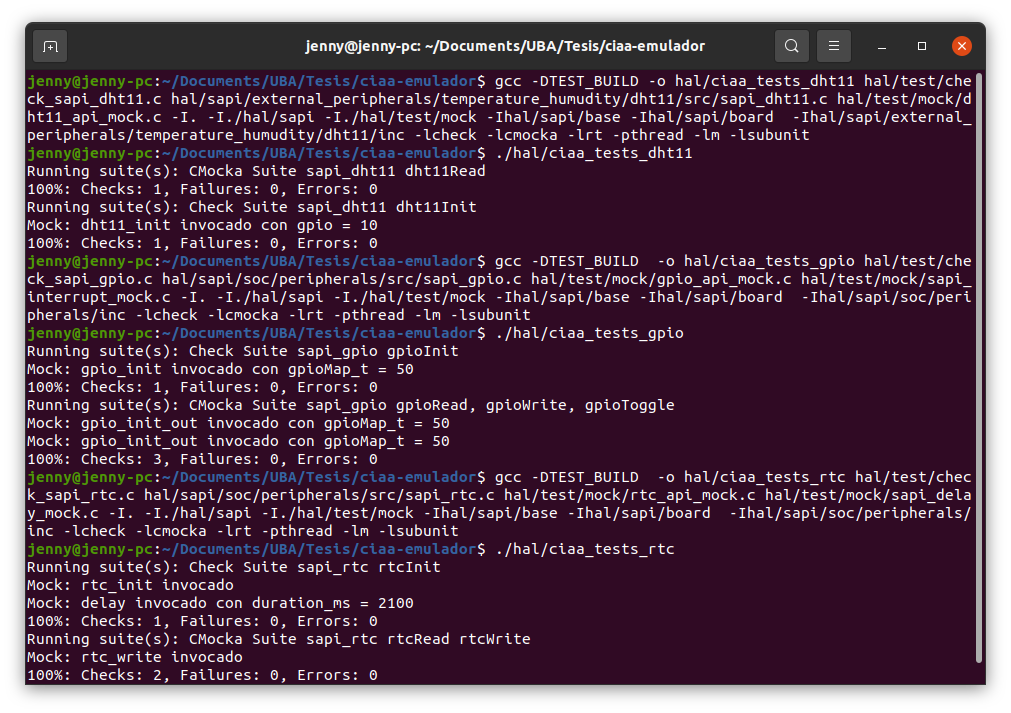
\includegraphics[scale=.27]{./Figures/PruebasUnidad1.png}
	\caption{Primera parte de la depuración de las pruebas unitarias con \textit{CMocka} o \textit{Check}.}
	\label{fig:PruebasUnidad1}
\end{figure}


\begin{figure}[ht]
	\centering
	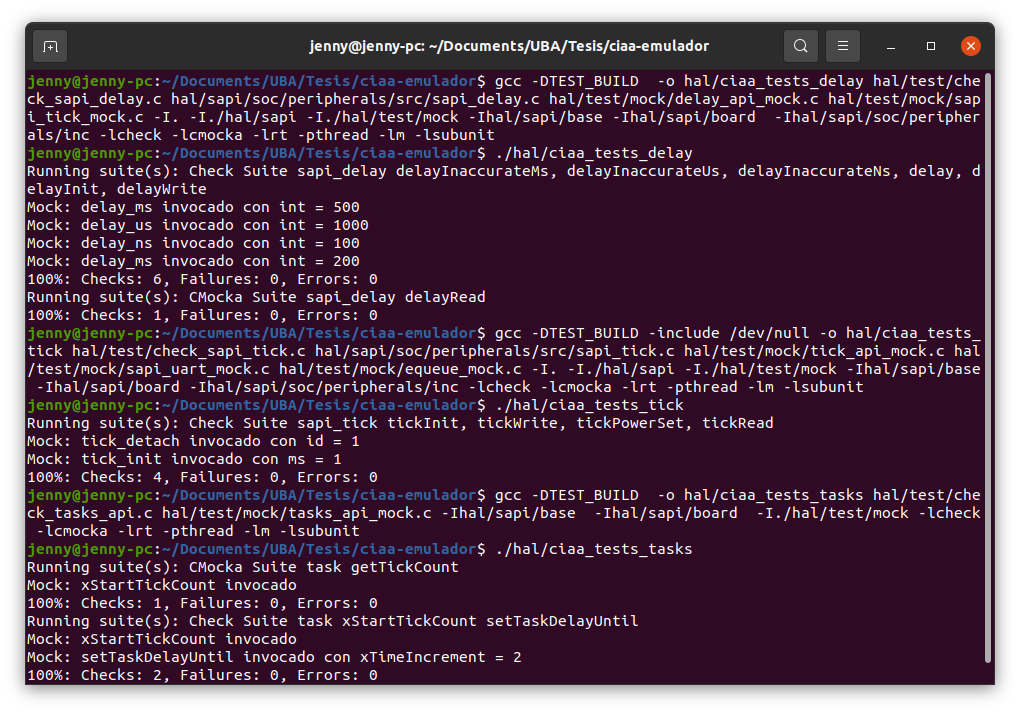
\includegraphics[scale=.27]{./Figures/PruebasUnidad2.png}
	\caption{Segunda parte de la depuración de las pruebas unitarias con \textit{CMocka} o \textit{Check}.}
	\label{fig:PruebasUnidad2}
\end{figure}
 

\section{Pruebas de Integración} 
\label{subsec:Pruebas de Integración}

Las pruebas de integración se centran en evaluar la interacción y comunicación entre diferentes componentes. Además, asegura que trabajen en conjunto sin problemas.

A medida que se fueron desarrollando diferentes módulos y funcionalidades del emulador, las pruebas de integración fueron necesarias para identificar posibles conflictos o incompatibilidades entre los distintos componentes de código del emulador web.

Se fueron identificando las interacciones entre componentes que fueron relevantes relevantes a partir de las pruebas de unidad existentes, como sapi\_delay y sapi\_tick. Luego, se identificaron las dependencias de emscripten y las funciones que se invocan entre las diferentes pruebas de unidad.

Luego, se crearon archivos de prueba de integración con escenarios especificos que  combinen las interacciones entre los componentes y se utilizaron mocks para simular comportamientos de funciones de emscripten .

la interacción con el usuario así como también con las peticiones hacia el backend.

Al igual que en las pruebas de unidad se utilizo el compilador GCC para compilar los archivos de código relevantes y cualquier dependencia necesaria.

A continuacion se muestra los resultados por consola


delays con ticks
gpio con interrupciones

En la figura \ref{fig:PruebasIntegracion} muestra la depuración de las pruebas de integracion.
\begin{figure}[ht]
	\centering
	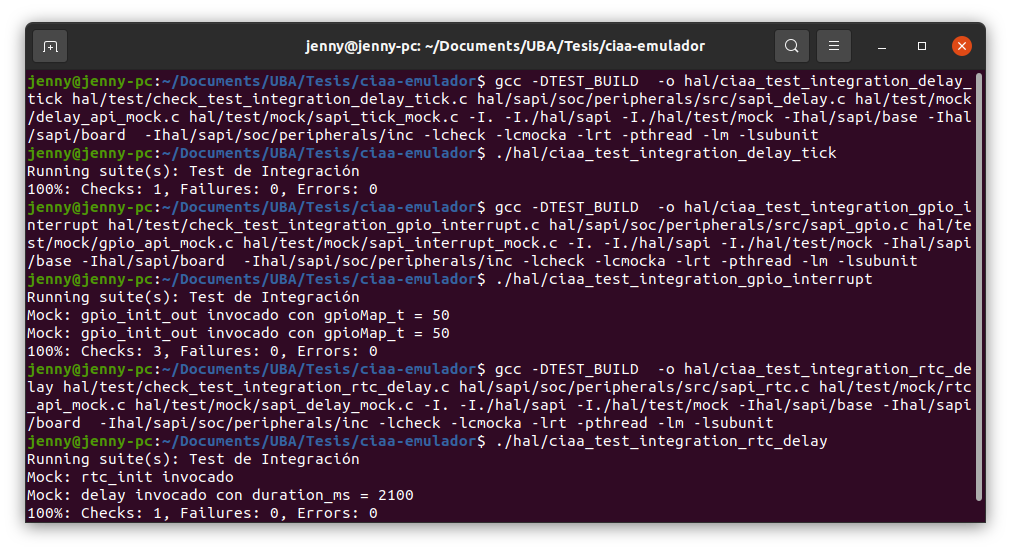
\includegraphics[scale=.35]{./Figures/PruebasIntegracion.png}
	\caption{Depuración de las pruebas de integracion.}
	\label{fig:PruebasIntegracion}
\end{figure}

Ademas, para probar codigo desde el fronted y el backend, se realizo prueba de ejecucion del boton ejecutar de la interfaz, con ello se realiza el programa.



\section{Pruebas de Interfaz}
\label{sec:Pruebas de Interfaz}

Para lograr que la interfaz de la plataforma de emulación cumpla con los requisitos funcionales y logre que los usuarios lo adopten con éxito fue necesario implementar las pruebas de la interfaz de usuario.

Por tanto, se implementaron pruebas automatizadas que verifiquen que el funcionamiento sea el correcto, tanto desde la interacción con el usuario así como también con las peticiones hacia el backend.

La implementación de pruebas automatizadas permitió ejecutarlas de forma rápida y confiable de manera recurrente. 

Para automatizar las pruebas de la interfaz de usuario con \textit{\textbf{NodeJS}}, el desarrollo se hizo mediante las bibliotecas \textit{\textbf{Mocha}} y \textit{\textbf{Chai}}, que permitieron crear pruebas unitarias muy completas para el desarrollo en JavaScript.

Además, permitió asegurar que cada módulo de la interfaz funcione correctamente por separado. Incluso, verificó si el código en el navegador web devolvió los nombres de los módulos correctos, los tipos de parámetros previstos y el tipo de retorno esperado.


La figura \ref{fig:TestVS1} muestra la primera parte de la depuración de las pruebas unitarias de \textit{\textbf{Mocha}}  en \textit{\textbf{Visual Studio Code}}.

\begin{figure}[ht]
	\centering
	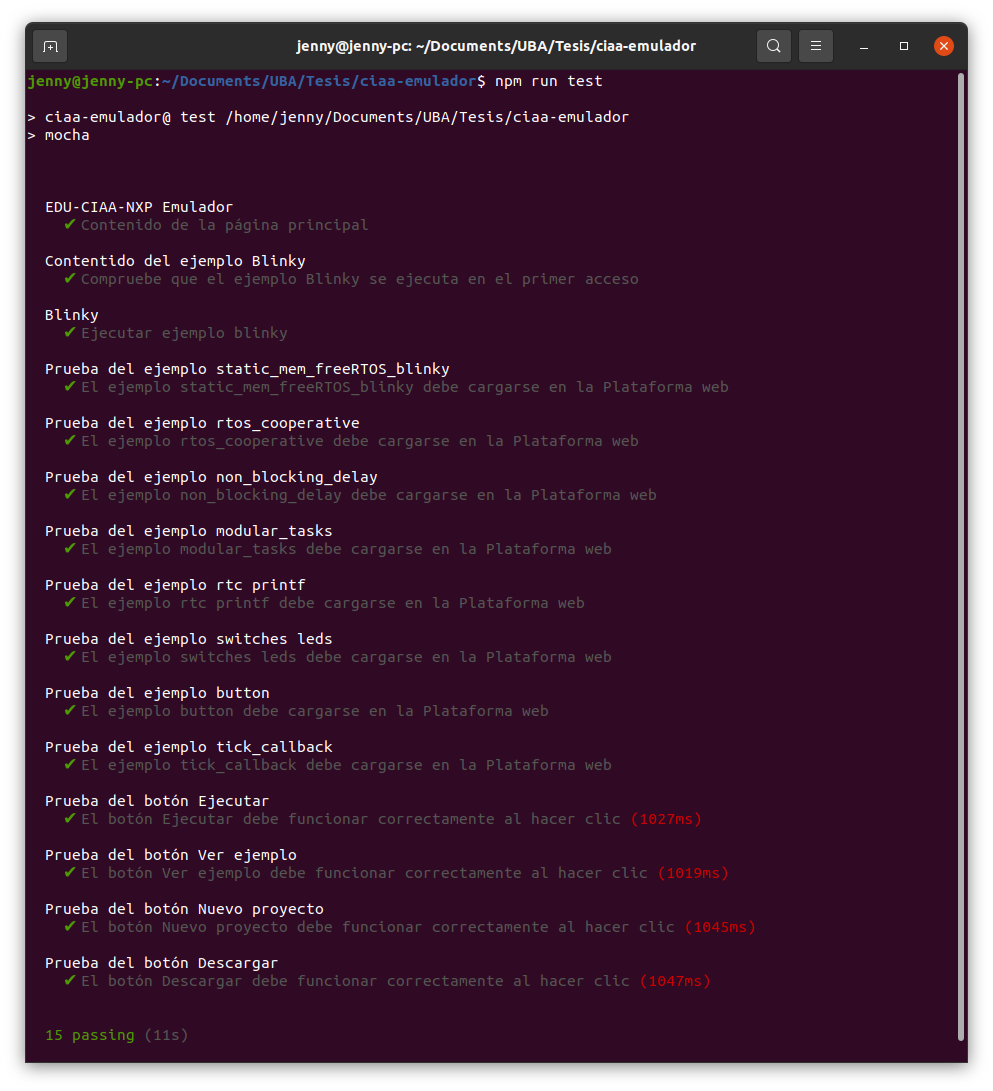
\includegraphics[scale=.29]{./Figures/TestInterfaz.png}
	\caption{Primera parte de la depuración de las pruebas unitarias.}
	\label{fig:TestVS1}
\end{figure}

\section{Integracion Continua}
\label{sec:Integracion Continua}

En la realizacion
no tenia en claro cual de las dos herramientas utilizar entonces se elijio ensayar ambas, las cuales dieron excelentes resultados y se pueden utilizar de forma intercambiable.
Diferencias: en una tengo que configurar todo en gitlab

El esfuerzo ya estaba hecho

Travis ci

Gitlab

\section{Pruebas de Validación}
\label{sec:Pruebas de Validación}

\section{Banco de pruebas}

Para verificar el funcionamiento de la plataforma de emulación se emplearon diversos recursos de software y hardware, que permitió una evaluación completa del funcionamiento de la plataforma de emulación, garantizando su confiabilidad y funcionalidad. 

El proceso de verificación incluyó también pruebas comparativas entre la plataforma de emulación y la placa física, donde se ejecutaron casos de prueba idénticos en ambos entornos. Esto permitió identificar y analizar las diferencias entre el comportamiento del emulador web y la real real, proporcionando información valiosa para mejorar la precisión y fiabilidad de la plataforma web de emulación.



En la tabla \ref{tab:RecursosHardware} se presentan los recursos de hardware empleados en el banco de pruebas.

\begin{table}[h]
	\centering
	\caption[Recursos de hardware utilizados]{Recursos de hardware utilizados.}
	\begin{tabular}{l c}    
		\toprule
		\textbf{Herramienta} & \textbf{Propósito}\\
		\midrule
		Computadora & Acceso a la plataforma de emulación.\\		
		Placa EDU-CIAA-NXP &  Implementación de los ejemplos de la sAPI.\\
		Dht11 temperature \& humidity  &  Pruebas de ejemplo.\\
		\bottomrule
		\hline
	\end{tabular}
	\label{tab:RecursosHardware}
\end{table}


Asimismo, se utilizaron herramientas de software para realizar las pruebas
en todos los módulos que componen el sistema. En la tabla \ref{tab:RecursosSoftware} se describe el propósito de estas herramientas.

\begin{table}[h]
	\centering
	\caption[Recursos de software utilizados]{Recursos de software utilizados.}
	\begin{tabular}{l c}    
		\toprule
		\textbf{Herramienta} & \textbf{Propósito}\\
		\midrule
		Mocha &  Pruebas automatizadas para el frontend.\\		
		Chai &   Pruebas automatizadas para el frontend.\\
		Chrome & Pruebas de la plataforma web.\\
		Firefox & Pruebas de la plataforma web.\\
		Explorer &  Pruebas de la plataforma web. \\
		PostMan \citep{Postman} &  Pruebas de \textit{request} de la plataforma y APIs. \\
		Gtest &  Pruebas automatizadas para el backend. \\
		Make \citep{Make} &  Para gestión de dependencias en las pruebas de backend. \\
				CTest \citep{CTest} &  Para la ejecución de las pruebas de backend. \\
Tera Term \citep{TeraTerm}		&  Emulador de la terminal serial. \\
		\bottomrule
		\hline
	\end{tabular}
	\label{tab:RecursosSoftware}
\end{table}



\section{Casos de uso}    
\label{sec:CasoUso}     

En esta sección se realiza el análisis de algunos casos de prueba y se muestran los resultados obtenidos. 

\subsection{Prueba de acceso}    

ID Caso de prueba: CP01 

Descripción: la primera vez que el usuario ingresa a la plataforma de emulación se muestra ejecutado el ejemplo predeterminado \textit{\textbf{Blinky}}.

Pre-condición: 
\begin{itemize}
	\item La computadora del usuario tiene una conexión a internet.
\end{itemize}

Flujo principal:
\begin{itemize}
	\item El usuario ingresa al entorno web de la plataforma de emulación para la placa EDU-CIAA-NXP.
\end{itemize}
Post condiciones:
\begin{itemize}
	\item ÉXITO: la plataforma muestra el ejemplo \textit{\textbf{Blinky}} en ejecución.
	\item FALLA: La plataforma no muestra ningún ejemplo predeterminado en ejecución.
\end{itemize}

Resumen del Test:
\begin{itemize}
	\item Después de acceder a la plataforma mediante los navegadores web Chrome, Firefox y Explorer se comprobó que se muestra en ejecución el ejemplo \textit{\textbf{Blinky}}.
	\item Se realizó la prueba de HTTP \textit{requests} por medio de la utilización de la herramienta \textit{\textbf{Postman}} que luego de acceder a la dirección donde se encuentra alojada la plataforma, devolvió en formato \textit{\textbf{JSON}} la respuesta del servidor.
\end{itemize}


La figura \ref{fig:PlataformaEmuladorBlinky} muestra la plataforma de emulación ejecutando el ejemplo predeterminado \textit{\textbf{Blinky}}.

\begin{figure}[ht]
	\centering
	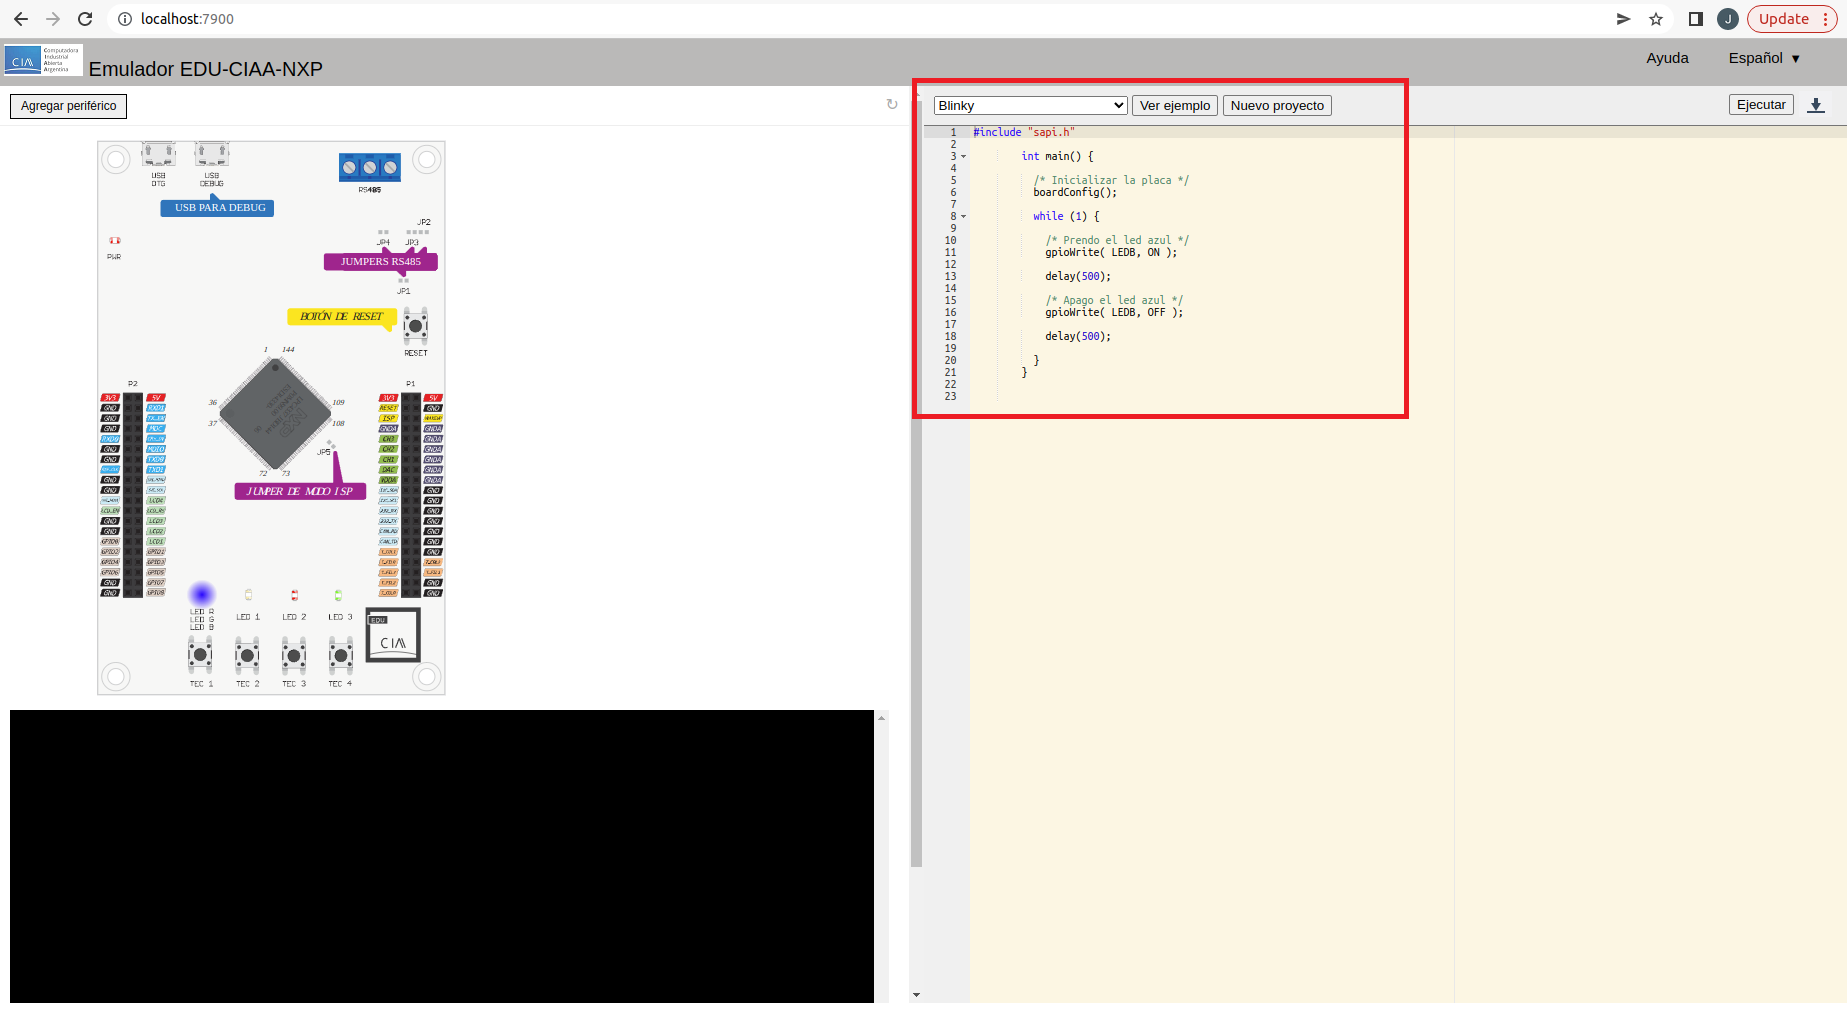
\includegraphics[scale=.21]{./Figures/PlataformaEmuladorBlinky.png}
	\caption{Prueba plataforma emulador ejecutando el ejemplo \textit{\textbf{Blinky}}.}
	\label{fig:PlataformaEmuladorBlinky}
\end{figure}

\textit{\textbf{Postman}} es una aplicación que permite realizar pruebas API. Con este cliente \textit{\textbf{HTTP}} se probó \textit{\textbf{HTTP requests}} que permitió el acceso a la plataforma de emulación y por medio de la cual se obtuvo la respuesta en diferentes formatos como  \textit{\textbf{JSON}}, \textit{\textbf{XML}}, \textit{\textbf{HTML}} y \textit{\textbf{Text}}.


En la figura \ref{fig:PostmanBlinky3} se muestra la petición de acceso a la plataforma por medio de la herramienta \textit{\textbf{Postman}}.

\begin{figure}[ht]
	\centering
	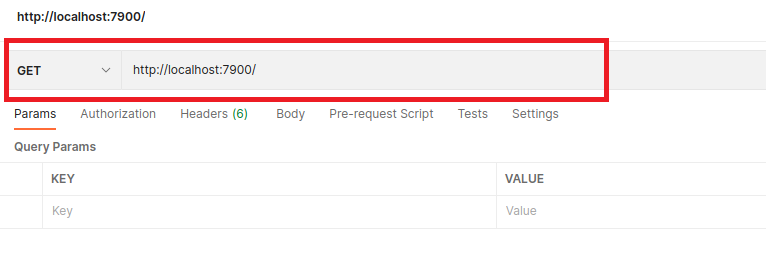
\includegraphics[scale=.50]{./Figures/PostmanBlinky3.png}
	\caption{Petición de acceso a la plataforma.}
	\label{fig:PostmanBlinky3}
\end{figure}




En la figura \ref{fig:PostmanBlinky2} se muestra la respuesta a la petición de acceso de la plataforma por medio de la herramienta \textit{\textbf{Postman}}.

\begin{figure}[ht]
	\centering
	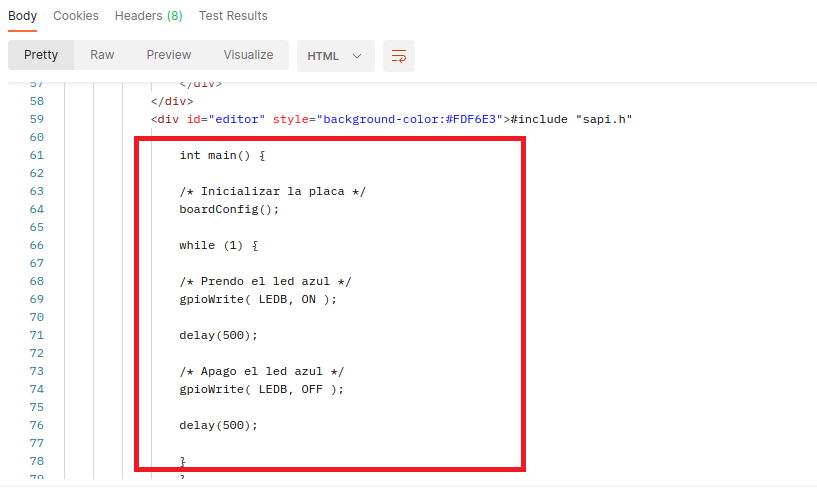
\includegraphics[scale=.37]{./Figures/PostmanBlinky2.png}
	\caption{Respuesta del servidor.}
	\label{fig:PostmanBlinky2}
\end{figure}

\hfill \break
\hfill \break

\subsection{Pruebas de precisión}  
Comparar la precisión de los cálculos realizados por el microcontrolador en la plataforma web con los resultados obtenidos en la placa física.

\subsection{Prueba de funcionamiento}    

ID Caso de prueba: CP02 

Descripción: la plataforma de emulación permite al usuario ejecutar el ejemplo \textit{\textbf{Dht11 temperature/humidity}}.

Pre-condición: 
\begin{itemize}
	\item La computadora del usuario tiene una conexión a internet.
\end{itemize}

Flujo principal:
\begin{itemize}
	\item El usuario ingresa al entorno web de la plataforma de emulación para la placa EDU-CIAA-NXP.
	\item El usuario selecciona desde la lista desplegable el ejemplo \textit{\textbf{Dht11 temperature/humidity}} y hace click en el botón "Ver ejemplo".
	\item La plataforma muestra en pantalla al usuario el código del ejemplo \textit{\textbf{Dht11 temperature/humidity}}.
	\item El usuario hace click en el botón “Agregar periférico”.
	\item La plataforma muestra al usuario una nueva ventana con una lista desplegable de selección de  periféricos.
	\item El usuario selecciona la opción "temperature/humidity".
	\item La plataforma muestra en el área de ensamblado el componente \textit{\textbf{Dht11 temperature/humidity}} junto a la placa EDU-CIAA-NXP.
	\item El usuario hace click en botón “Ejecutar”.
	\item La plataforma muestra los cambios en la placa EDU-CIAA-NXP y en la terminal de salida.
\end{itemize}
Post condiciones:
\begin{itemize}
	\item ÉXITO: la plataforma muestra en ejecución el ejemplo \textit{\textbf{Dht11 temperature/humidity}}.
	\item FALLA: La plataforma no muestra al usuario ningún cambio en pantalla.
\end{itemize}

Resumen del Test:
\begin{itemize}
	\item Después de acceder a la plataforma mediante los navegadores web Chrome, Firefox y Explorer se comprobó que se muestra en ejecución el ejemplo \textit{\textbf{Dht11 temperature/humidity}}.
	\item Se implementó en la placa real EDU-CIAA-NXP  el mismo ejemplo \textit{\textbf{Dht11 temperature/humidity}} y se registraron los resultados.
	\item Se realizó la prueba de HTTP \textit{requests} usando la herramienta \textit{\textbf{Postman}} para comprobar la respuesta del \textit{\textbf{API openweathermap}} que consume la plataforma de emulación de manera que, los datos de temperatura y humedad sean los mismos.
\end{itemize}

\subsubsection{Ensayo en la plataforma EDU-CIAA-NXP} 

Este ensayo tuvo como objetivo identificar
las diferencias entre los resultados reales producidos por la placa real y los resultados esperados en la plataforma de emulación.

El primer paso fue conectar el componente Dht11 a la placa EDU-CIAA-NXP. En consecuencia, se procedió a compilar el ejemplo \textit{\textbf{Dht11 temperature/humidity}} de la plataforma de emulación dentro de la herramienta 
\textit{Eclipse} y luego, se grabó en la placa EDU-CIAA-NXP.

A continuación se muestra en la figura \ref{fig:TestHardware} la ejecución del ensayo en la plataforma EDU-CIAA-NXP.

\begin{figure}[ht]
	\centering
	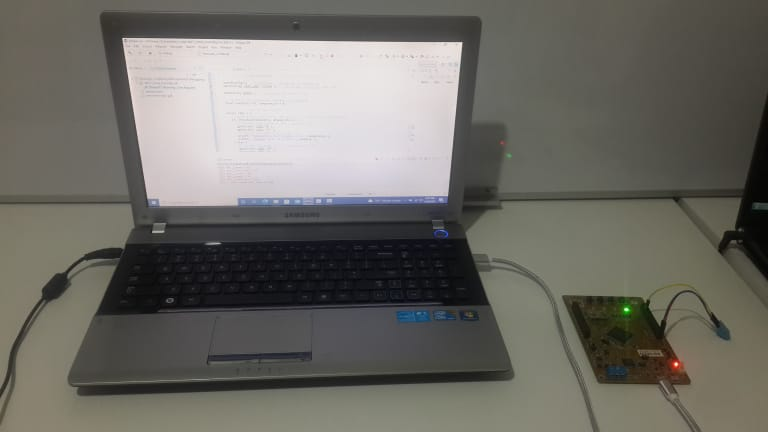
\includegraphics[scale=.49]{./Figures/TestHardware.jpeg}
	\caption{Ensayo del ejemplo \textit{\textbf{Dht11 temperature/humidity}}.}
	\label{fig:TestHardware}
\end{figure}



La figura \ref{fig:TestEclipse} muestra el código del ejemplo \textit{\textbf{Dht11 temperature/humidity}} en la herramienta \textit{eclipse} de la PC de prueba.

\begin{figure}[ht]
	\centering
	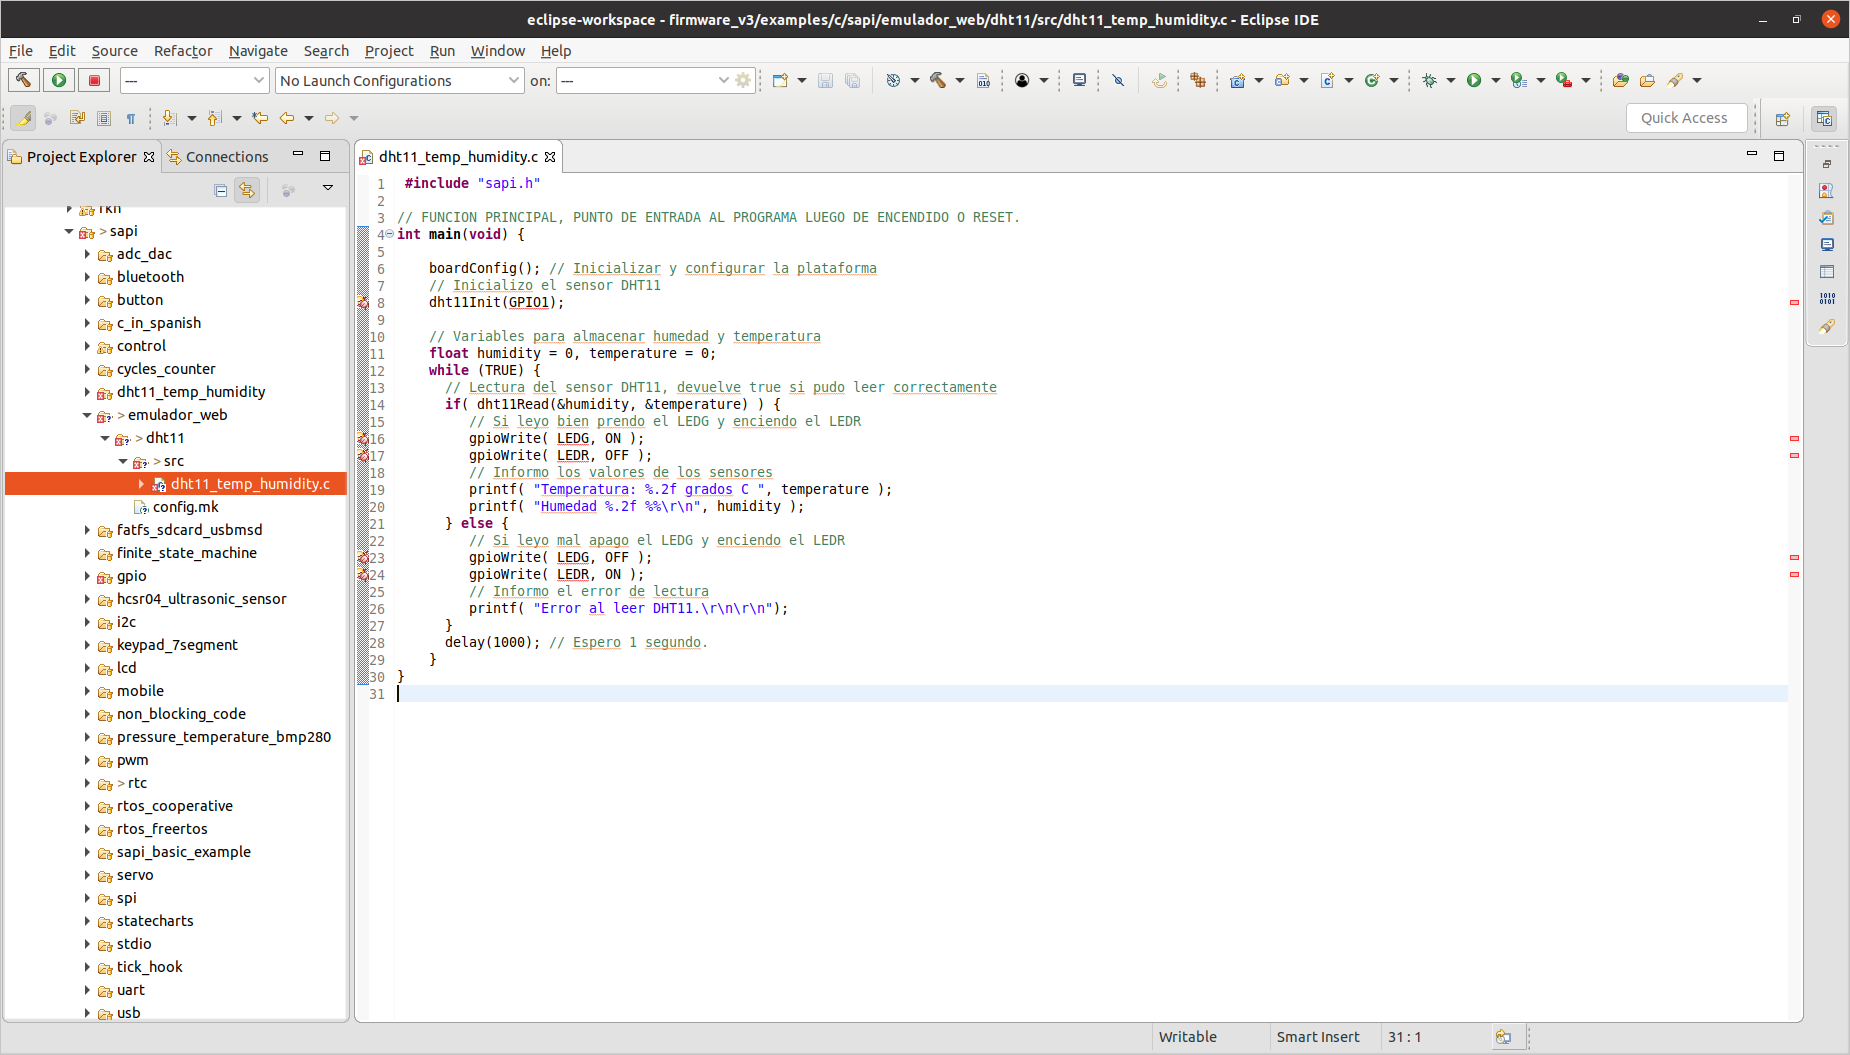
\includegraphics[scale=.22]{./Figures/TestEclipse.png}
	\caption{Código del ejemplo en eclipse.}
	\label{fig:TestEclipse}
\end{figure}

\hfill \break
\hfill \break
\hfill \break
\hfill \break

El programa \textit{\textbf{Dht11 temperature/humidity}} de la plataforma de emulación es un ejemplo simple que solo enciende el LEDG en la placa y además, lee los datos generados del sensor Dht11 que consisten en temperatura/humedad. Luego, los datos leídos se imprimen por pantalla. 

En este ensayo manual se registraron los cambios en la placa y también, los mensajes de la terminal serie. De modo que, posteriormente, permitió compararlos con la plataforma de emulación.

En la figura \ref{fig:TestPlaca} se observan los cambios en la placa que fueron registrados durante las pruebas.


\begin{figure}[ht]
	\centering
	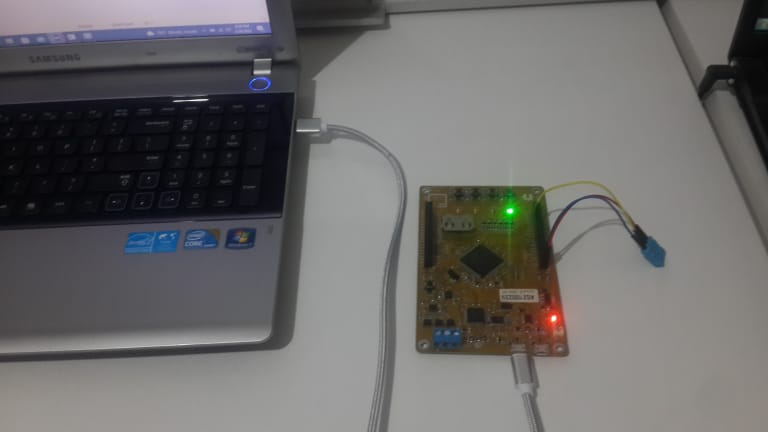
\includegraphics[scale=.50]{./Figures/TestPlaca.jpeg}
	\caption{Cambios en la placa EDU-CIAA-NXP durante el ensayo.}
	\label{fig:TestPlaca}
\end{figure}


Ahora bien, para leer los datos por pantalla se utilizó la herramienta \textit{Tera Term VT} que permitió levantar los datos de temperatura/humedad.

En la figura \ref{fig:TestTerminal} se muestra los datos de temperatura/humedad usando \textit{Tera Term VT}. 


\begin{figure}[ht]
	\centering
	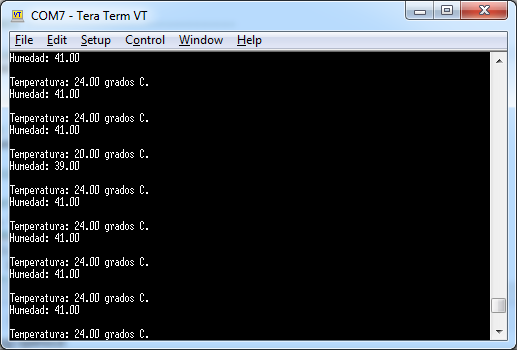
\includegraphics[scale=.59]{./Figures/TestTerminal.png}
	\caption{Salida de la terminal COM8 -Tera Term VT.}
	\label{fig:TestTerminal}
\end{figure}

\subsubsection{Ensayo en la plataforma de emulación para la placa EDU-CIAA-NXP} 

Después de registrar los resultados del ensayo del programa \textit{\textbf{Dht11 temperature/humidity}} en la plataforma real de la placa EDU-CIAA-NXP, se continuó con el ensayo en la plataforma de emulación siguiendo los pasos del caso de uso CP02.

En consecuencia, luego de completar el último paso y llegar a la post condición se obtuvo el siguiente resultado: 

\begin{itemize}
	\item ÉXITO: la plataforma muestra en ejecución el ejemplo \textit{\textbf{Dht11 temperature/humidity}}.
\end{itemize}

La figura \ref{fig:RespuestaEmulador} muestra en ejecución el ejemplo \textit{\textbf{Dht11 temperature/humidity}}.


\begin{figure}[ht]
	\centering
	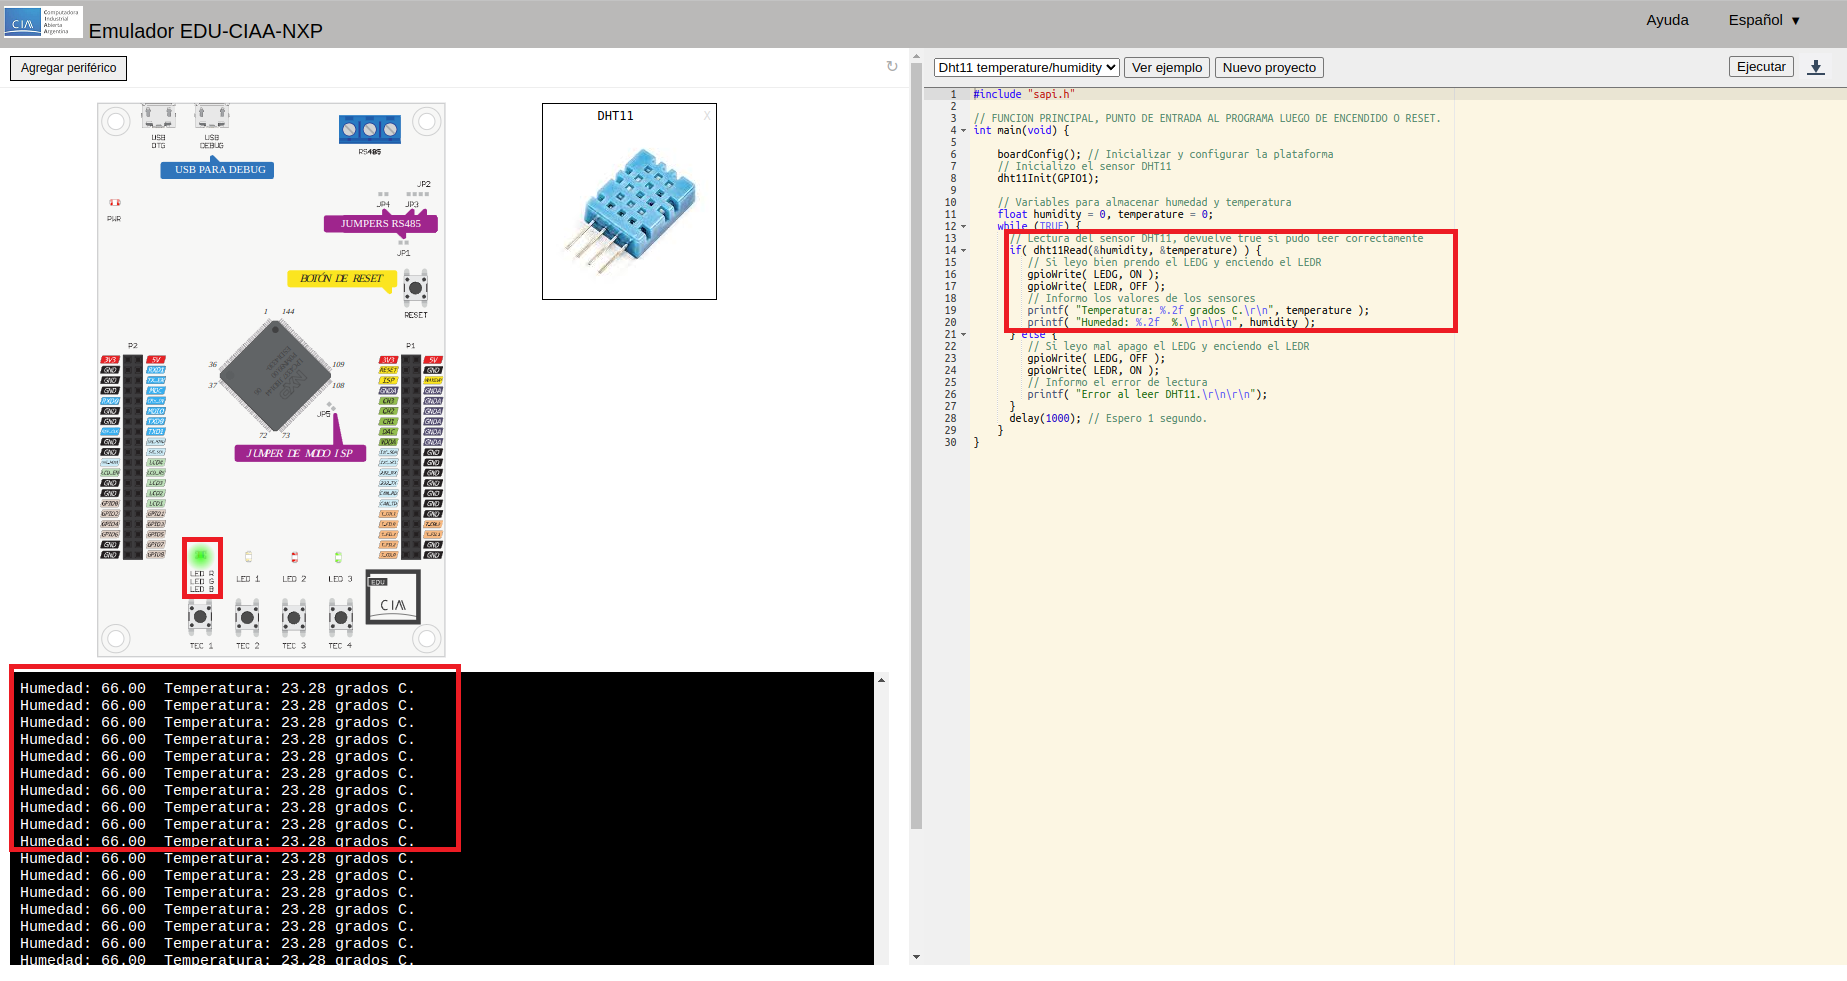
\includegraphics[scale=.21]{./Figures/RespuestaEmulador.png}
	\caption{La plataforma muestra el resultado del CP02.}
	\label{fig:RespuestaEmulador}
\end{figure}


Primero, se verificó que el ejemplo \textit{\textbf{Dht11 temperature/humidity}} es el que se utilizó para el ensayo en la plataforma real EDU-CIAA-NXP.

En la figura \ref{fig:RespuestaEmulador2} se puede observar el ejemplo \textit{\textbf{Dht11 temperature/humidity}} ejecutado en la plataforma de emulación.


\begin{figure}[ht]
	\centering
	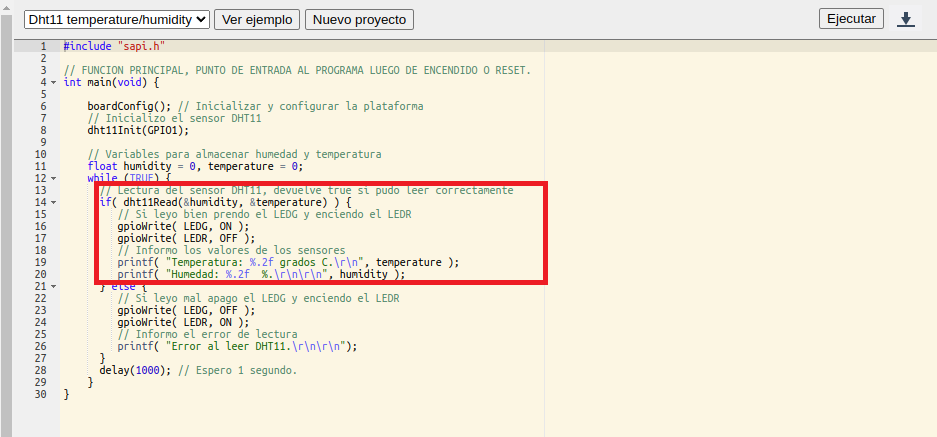
\includegraphics[scale=.41]{./Figures/RespuestaEmulador2.png}
	\caption{Ejemplo \textit{\textbf{Dht11 temperature/humidity}} ejecutado en la plataforma de emulación.}
	\label{fig:RespuestaEmulador2}
\end{figure}


En segundo lugar, se verificó la salida de los datos de temperatura/humedad en la terminal serie.  

Cabe destacar que para imitar los datos generados del sensor de temperatura/humedad, la plataforma de emulación se conecta al API de meteorología  \textit{\textbf{openweathermap}} que permite obtener datos meteorológicos de una región en particular. De manera que, la plataforma de emulación muestra la temperatura y humedad de la ciudad/país desde donde se accede a la plataforma web.

En la figura \ref{fig:RespuestaEmulador1} se pueden observar los datos de temperatura/humedad devueltos por la plataforma de emulación.


\begin{figure}[ht]
	\centering
	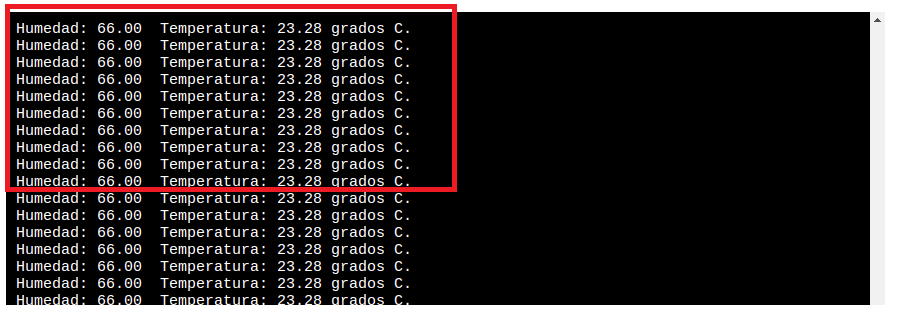
\includegraphics[scale=.43]{./Figures/RespuestaEmulador1.png}
	\caption{Datos de temperatura/humedad mostrados por la plataforma.}
	\label{fig:RespuestaEmulador1}
\end{figure}


Para verificar que la plataforma obtuvo los datos de temperatura/humedad del API de meteorología  \textit{\textbf{openweathermap}} se hicieron pruebas de request con la herramienta \textit{Postman}.

En la figura \ref{fig:RespuestaPostMan1} se observa que la petición de datos de temperatura/humedad recibe como parámetro la ciudad que se quiere consultar.
\begin{figure}[ht]
	\centering
	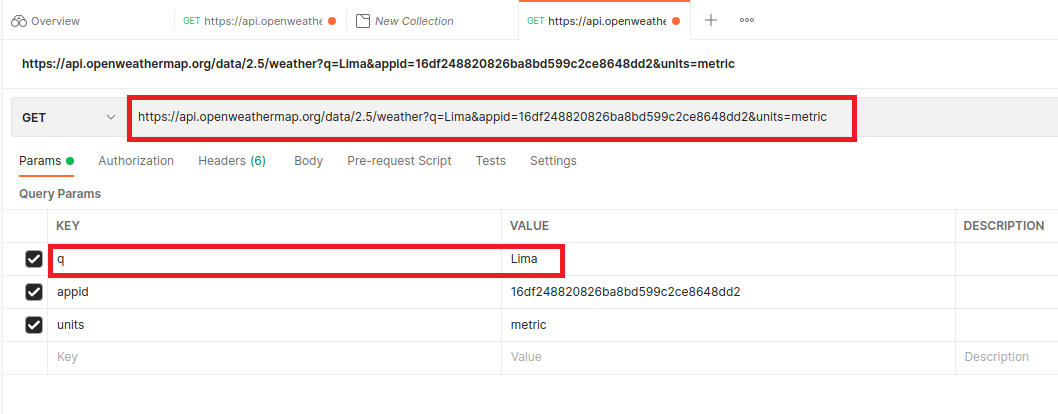
\includegraphics[scale=.36]{./Figures/RespuestaPostMan1.png}
	\caption{Petición de datos de temperatura/humedad.}
	\label{fig:RespuestaPostMan1}
\end{figure}

En este paso se verifica que la respuesta de la petición de datos de temperatura/humedad al API \textit{\textbf{openweathermap}} coincide con lo que se observó en la terminal de la plataforma de emulación.

En la figura \ref{fig:RespuestaPostMan2} se observa la repuesta de la petición de datos de temperatura/humedad de la herramienta \textit{Postman}.
\begin{figure}[ht]
	\centering
	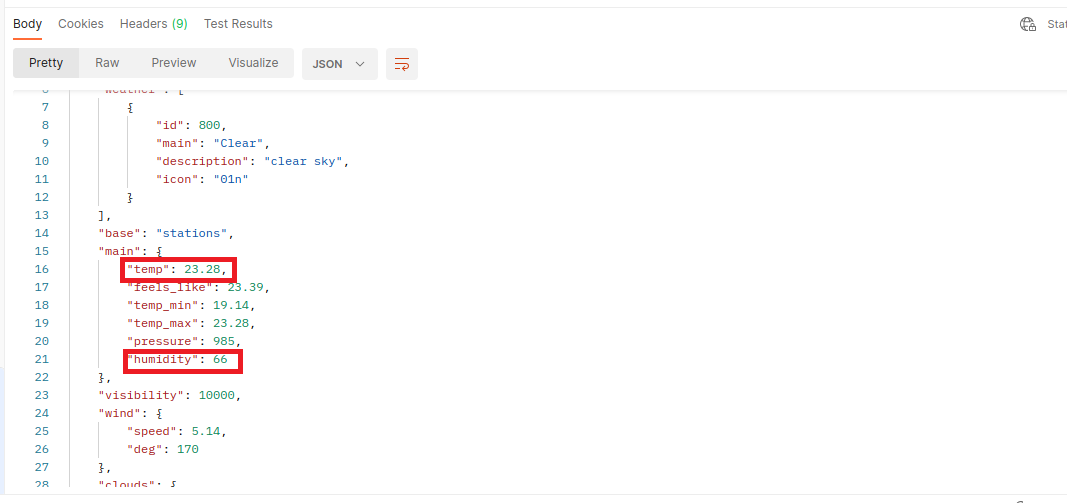
\includegraphics[scale=.36]{./Figures/RespuestaPostMan2.png}
	\caption{Repuesta de la petición de datos de temperatura/humedad.}
	\label{fig:RespuestaPostMan2}
\end{figure}


Como último paso se verificó que los cambios en la placa coinciden con los que se registraron en la plataforma real de la placa EDU-CIAA-NXP. En consecuencia, se observó encendido el LEDG.

\hfill \break
\hfill \break
\hfill \break
\hfill \break
\hfill \break
\hfill \break
\hfill \break
\hfill \break


En la figura \ref{fig:RespuestaLed} se observan los cambios en la placa EDU-CIAA-NXP de la plataforma de emulación.

\begin{figure}[ht]
	\centering
	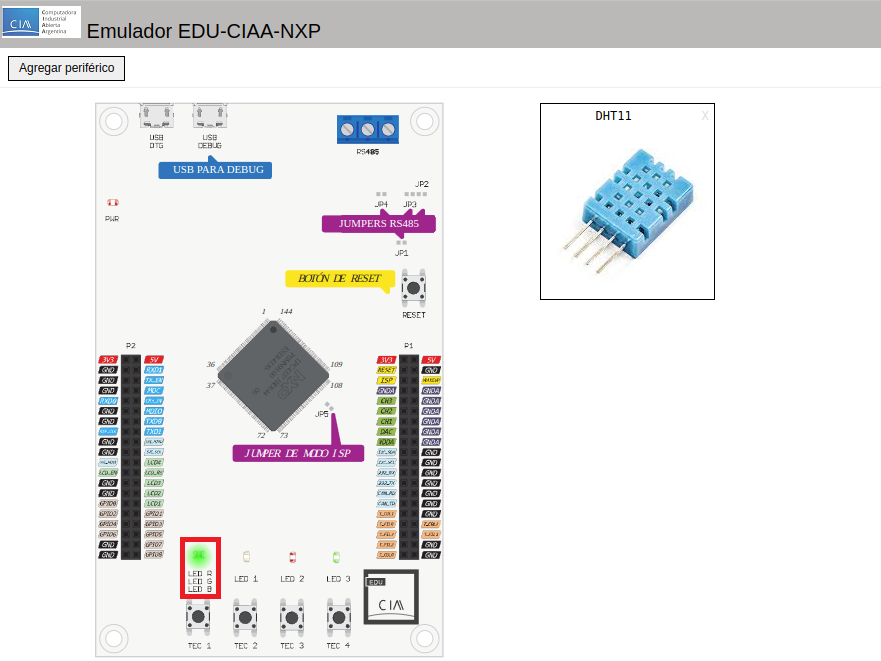
\includegraphics[scale=.43]{./Figures/RespuestaLed.png}
	\caption{Cambios en la placa EDU-CIAA-NXP durante el ensayo.}
	\label{fig:RespuestaLed}
\end{figure}
